\documentclass[11pt]{article}
\usepackage[T1]{fontenc}
\usepackage[utf8]{inputenc}
\usepackage{lmodern}
\usepackage[margin=1in]{geometry}
\usepackage{microtype}
\usepackage{amsmath}
\usepackage{booktabs}
\usepackage{array}
\newcolumntype{L}[1]{>{\raggedright\arraybackslash}p{#1}}
\usepackage{graphicx}
\usepackage{enumitem}
\usepackage[numbers,sort&compress]{natbib}
\usepackage{xurl}
\usepackage[hidelinks]{hyperref}
\usepackage{caption}
\captionsetup{font=small,labelfont=bf}
\setlist{itemsep=2pt,topsep=4pt}

\title{Meeting a Definition of Recursive Self-Improvement Is Not Evidence That the Recursion Helps:\\[2pt]
\large A Preregistered Test with Counterfactual Controls}
\author{Junai P.\ Felix\\
\small Independent Researcher, Taipei, Taiwan\\
\small \texttt{junai.felixx@gmail.com}}
\date{October 2026}

\begin{document}
\maketitle

\begin{abstract}
Claims of recursive self-improvement (RSI) are usually judged against criteria their authors choose, and recent capability taxonomies grade systems by which roles they perform. We test whether satisfying such a definition shows that the recursion is productive. A self-modifying program-repair runtime, FELIX-C3, was tested against the published Level-4 definition of bounded RSI of Liu et al.\ (2026). Its improvement mechanism is an explicit, versioned object that contains the procedure for editing itself. Definition, criteria, seeds and gates were registered before any code was written; the build was frozen and hashed; the confirmatory experiment ran once (24 unused seeds $\times$ 3 conditions, 32 rounds, no operator). Every definitional criterion passed: validated rewrites of the mechanism were adopted in 21 of 24 missions, the rewriting procedure rewrote itself in 17, and test solve rate rose from 27.4\% to 40.1\% with significant second-half progress ($p = 7.6\times10^{-6}$). The counterfactual criteria failed: rewriting did not beat the same system with its mechanism frozen ($+0.35$ pp, $p = 0.23$) or with rewrites adopted by coin flip ($+0.72$ pp, $p = 0.079$). Four further preregistered studies, including a noise-aware redesign whose rewrites did worse than the default ($-1.12$ pp), did not change this. A companion preregistered study found that the system's policies repair 23\% more real bugs from QuixBugs and HumanEvalFix than its starting policy ($p = 3.0\times10^{-7}$), equally under all three conditions. A system can therefore meet a Level-4 definition while its recursion contributes nothing measurable. We propose that RSI claims report matched-budget frozen-mechanism and random-adoption controls with a power analysis, and we release per-seed data, a reanalysis that reproduces the reported statistics, and a preregistration draft for three follow-up tests.
\end{abstract}

\section{Introduction}

A system exhibits recursive self-improvement when it improves the procedure by which it improves itself \cite{good1966,schmidhuber2003}. Empirical systems now revise their own scaffolds, agent designs and code \cite{zelikman2024stop,yin2025godel,hu2025adas,zhang2026dgm,robeyns2025sica,wang2026hgm}, and the word ``recursive'' is applied to many of them. Two recent surveys supply external yardsticks. Liu et al.\ \cite{liu2026path} grade self-improving agents on five levels; at Level~4, \emph{bounded recursive self-improvement}, a system rewrites its own improvement mechanism and sustains long-term progress within a bounded domain. Chen et al.\ \cite{chen2026rsi} separate bounded self-refinement against fixed evaluators from open-ended RSI. Both treat rewriting the improvement mechanism as the step that separates recursion from ordinary self-modification.

Such definitions are written to classify architectures: they ask which roles a system performs. They do not ask whether performing the recursive role helps. This paper reports a test designed to separate the two questions. We built a system whose improvement mechanism is an explicit object that rewrites itself, translated each clause of the Level-4 definition into a preregistered criterion, and added two criteria the definition does not require: a frozen-mechanism control and a random-adoption control at matched budget.

The result is a clean dissociation. The system meets every clause of the definition, and its recursion contributes nothing measurable. Four follow-up preregistered studies that redesigned how rewrites are validated did not change this, and a companion study shows that the gains the system does make transfer to real bugs, equally with and without recursion.

\paragraph{Contributions.}
\begin{itemize}
\item A preregistered, single-attempt test of a self-modifying system against a published Level-4 RSI definition, with counterfactual controls at matched budget (\S\ref{sec:def}--\S\ref{sec:results}).
\item A dissociation: all definitional criteria pass, all counterfactual criteria fail, and five preregistered tests of productive recursion find none (\S\ref{sec:results}).
\item Evidence that the system's progress is real and partly transfers to real bugs, but comes from its improvement loop, not its recursion (\S\ref{sec:transfer}).
\item A reanalysis from the printed per-seed tables that reproduces the reported statistics, and a power analysis showing that a common ``significance plus minimum observed effect'' rule caps power near 57\% (\S\ref{sec:reanalysis}).
\item A proposed reporting standard for RSI claims (\S\ref{sec:discussion}) and a preregistration draft for three follow-up tests (\S\ref{sec:next}).
\end{itemize}

\paragraph{Relation to earlier reports.} This article consolidates two preprints by the author: the Stage~3 test, FELIX-C3 v1.3 \cite{felix2026c3}, and the transfer study, FELIX-C7 v1.1 \cite{felix2026c7}. Every experimental number here is reported there in full, with the complete design record. New in this article are the framing, the reanalysis and power analysis, the reporting proposal and the follow-up protocol.

\section{Background}

\paragraph{Recursive self-improvement.} Good framed RSI as improvement of the improver \cite{good1966}; Schmidhuber's G\"odel machine made it precise as self-rewriting under a proof obligation \cite{schmidhuber2003}; Yampolskiy surveyed its conceptual limits \cite{yampolskiy2015}. Learned optimisers \cite{andrychowicz2016} and evolved learning algorithms \cite{real2020automl} learn parts of the learning procedure, while the outer procedure usually stays fixed.

\paragraph{Empirical self-improving agents.} The Self-Taught Optimizer improves the scaffold that improves programs, including itself \cite{zelikman2024stop}. G\"odel Agent modifies its own logic at run time \cite{yin2025godel}. ADAS searches over agent code with a meta-agent \cite{hu2025adas}. The Darwin G\"odel Machine keeps an archive of coding agents that rewrite their own code \cite{zhang2026dgm}; the Self-Improving Coding Agent edits its own implementation \cite{robeyns2025sica}; the Huxley-G\"odel Machine guides self-modification by estimated descendant productivity \cite{wang2026hgm}. Liu et al.\ place several of these at Level~4 and none at Level~5 \cite{liu2026path}.

\paragraph{Preregistration.} Preregistration separates confirmatory from exploratory analysis \cite{nosek2018}; machine-learning results are sensitive to seeds and undisclosed analysis choices \cite{henderson2018,pineau2021}. We fix seeds, hold-out, conditions, statistics and pass rules before writing code and use exact nonparametric tests \cite{wilcoxon1945} with bootstrap intervals \cite{efron1979} as descriptive statistics.

\section{Target definition and operationalisation}\label{sec:def}

Liu et al.\ define Level~4 as follows \cite{liu2026path}:
\begin{quote}\small
``(L4) Bounded recursive self-improvement. The agent system can not only propose candidate modifications, validate their effects, and apply the validated modifications, but also rewrite its own improvement mechanism, which makes the improvement mechanism self-referential. Individual steps need not modify every component, but the overall process supports sustained long-term progress within a bounded domain.''
\end{quote}
The improvement mechanism \emph{Imp} ``governs how evidence and feedback are used to modify the agent system over time''. We wrote one criterion per clause (Table~\ref{tab:criteria}) and fixed every threshold before code existed. ``Rewrite its own improvement mechanism'' is read as the adoption of at least one validated change to an explicit Imp specification; ``self-referential'' is read structurally, so the procedure that rewrites Imp must itself be part of Imp; ``sustained long-term progress'' is read as significant improvement on fresh test tasks across the second half of long missions. Tier~B goes beyond the definition on purpose: only a frozen-mechanism counterfactual can tell a productive recursion from one that contributes nothing.

\begin{table}[t]
\centering\small
\caption{Preregistered criteria. Tier A operationalises the Level-4 definition; Tier B adds counterfactual controls. All refer to the live condition C6; $N=24$ missions; tests are one-sided exact Wilcoxon on per-seed paired differences.}
\label{tab:criteria}
\begin{tabular}{@{}lL{4.2cm}L{7.6cm}@{}}
\toprule
ID & Clause or question & Preregistered criterion\\
\midrule
A-1 & propose, validate, apply & An externally audited policy revision is promoted in $\ge 20$ of 24 missions.\\
A-2 & rewrite its own Imp & A validated Imp edit is adopted in $\ge 20$ of 24 missions.\\
A-3 & self-referential & The Imp-editing procedure lies inside the editable Imp (verified in the frozen source).\\
A-4 & sustained long-term progress & Test solve rate, round 32 minus round 16: mean $\ge +1.0$ pp and $p < 0.01$.\\
A-5 & integrity & Sources match the freeze; every mission reconciles, including its Imp hash chain.\\
\midrule
B-1 & Does rewriting Imp help? & Round 32, C6 $-$ C6f: mean $\ge +1.0$ pp and $p < 0.01$.\\
B-2 & Does evidence matter? & Round 32, C6 $-$ C6r: mean $\ge +1.0$ pp and $p < 0.05$.\\
\bottomrule
\end{tabular}
\end{table}

\section{System and design}\label{sec:design}

\paragraph{Disclosure boundary.} We describe the system at the level of roles, interfaces and parameter groups. The representation of the task policy, the vocabulary, the evidence format and the internal form of each Imp parameter are withheld. Everything needed to check the experiment against the definition is reported.

\paragraph{The improvement loop.} The domain is finite-grammar program repair: short programs with one to three injected faults, from 16 parametric families, four of which (\texttt{any\_neg}, \texttt{count\_gt}, \texttt{modwrap}, \texttt{poly}) are held out from all training and were derived from the freeze hash. Each round, the system diagnoses failures on a training batch, proposes vocabulary additions and 8 candidate policy revisions under the current Imp, screens them on 96 selection tasks, and sends the best to an external audit on 300 fresh tasks if it beats the incumbent. A candidate is promoted only if the audit shows a gain of at least 0.02 with a one-sided sign test $p \le 0.10$. Each task attempt is capped at 12 evaluations. Test checkpoints (320 tasks, 20 per family) at rounds 0, 16 and 32 are written to the mission state but never read by the system.

\paragraph{The improvement mechanism.} Imp is one structured object with 11 parameters in four groups: proposal (3), generation (4), screening (1) and the editing procedure (3: trial cadence, step size and adoption margin). When the round is a multiple of the incumbent's cadence, the system proposes a variant that changes one or two parameters, by an amount scaled by the incumbent's step size. For the next cadence rounds the per-round budget is split equally between the incumbent and the variant, whose vocabulary additions are isolated from each other; each round is a win, loss or tie for the variant by the mean solve count of each side's best two candidates. The variant is adopted if wins minus losses reach the incumbent's margin. Because step size, cadence and margin are read from the current Imp, the procedure that rewrites Imp is rewritten by itself. A trial exercises only the proposal and generation parameters; screening and editing-procedure changes act only after adoption.

\paragraph{Conditions.} Three conditions share the initial Imp, budget and task streams: \textbf{C6} (Imp rewritable on evidence), \textbf{C6f} (Imp frozen; the Level-3 counterfactual) and \textbf{C6r} (Imp rewritten on the same schedule with adoption by coin flip). Total evaluations per mission differed by less than 0.4\% between conditions.

\paragraph{Registration, freeze and gates.} The protocol was posted to a hosted document store with server timestamps before any code for this stage existed, followed by a freeze record (eight source hashes, configuration and initial Imp combined into one freeze hash), a gate record and a results record. Gate~0 checked determinism, distinct trajectories and headroom. Gate~1, an 8-seed pilot, returned GO for Tier~A and predicted the Tier~B outcome before the confirmatory run: the pilot C6 $-$ C6f difference was $+0.1$ pp and the bootstrap power for B-1 was 0.01. The confirmatory experiment ran once, on seeds 7101--7124, with no seed excluded.

\paragraph{Autonomy.} Every mission ran under a crash-only supervisor \cite{candea2003} with a lease, a watchdog, at most two restarts, atomic checksummed checkpoints and a hash-chained receipt per round. A 14-group fault suite injected faults in the middle of Imp trials, and eight deliberately broken supervisors tested whether the suite could fail \cite{demillo1978,jia2011}.

\section{Results}\label{sec:results}

\subsection{Every definitional criterion passes}

\begin{table}[t]
\centering\small
\caption{Tier A: confirmatory seeds 7101--7124, condition C6. Verdict: Level 4 (definitional).}
\label{tab:tierA}
\begin{tabular}{@{}lL{11.2cm}l@{}}
\toprule
ID & Result & \\
\midrule
A-1 & 24/24 missions promoted an audited revision (134 promotions) & pass\\
A-2 & 21/24 missions adopted a validated Imp edit (60 of 166 trials) & pass\\
A-3 & Editing procedure inside the editable Imp; in 17/24 missions an adopted edit changed it (25 of 60 edits) & pass\\
A-4 & Round 16 $\to$ 32: $+2.12$ pp, 95\% CI $[+1.33, +2.97]$; 18 up, 2 down, 4 unchanged; $p = 7.6\times10^{-6}$ & pass\\
A-5 & Sources match the freeze; 72/72 missions reconcile, including Imp hash chains & pass\\
\bottomrule
\end{tabular}
\end{table}

Table~\ref{tab:tierA} gives the outcome. Test solve rate under C6 rose from 27.4\% at round 0 to 38.0\% at round 16 and 40.1\% at round 32. Rewriting was not confined to the start: 31 of the 60 adoptions came in the second half. The mechanism did not lower its own bar: every first adoption was judged under the initial margin, and among adopted edits the margin rose three times and fell three times. All 72 confirmatory missions ran with zero interventions, restarts or watchdog kills; the frozen supervisor passed 14 of 14 fault groups, and each of the 8 broken supervisors failed at least one. During development the suite caught a real defect, a resume nondeterminism that made 7 of 14 groups fail, which was fixed before the freeze.

\subsection{Every counterfactual criterion fails}

\begin{figure}[t]
\centering
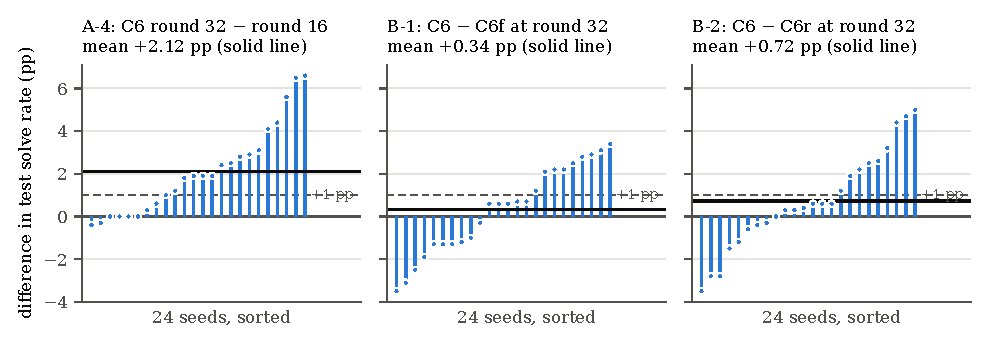
\includegraphics[width=\linewidth]{figures/fig1_stage3_paired.pdf}
\caption{Per-seed paired differences in test solve rate at round 32, computed from the printed per-seed table (\cite{felix2026c3}, Table 24; values rounded to 0.1 pp, so means can differ from the reported ones in the last digit). Left: second-half progress (A-4) passes. Middle and right: the counterfactual contrasts B-1 and B-2 straddle zero; neither reaches the $+1$ pp bar (dashed).}
\label{fig:stage3}
\end{figure}

Rewriting Imp on evidence did not produce a significantly better final policy than leaving Imp frozen (B-1: $+0.35$ pp, 95\% CI $[-0.47, +1.15]$, 14/10/0 seeds, $p = 0.23$), nor than rewriting it on the same schedule with adoption by coin flip (B-2: $+0.72$ pp, $[-0.14, +1.60]$, 15/8/1, $p = 0.079$); Figure~\ref{fig:stage3}. The decisive observation is that the frozen control also sustains progress: C6f gained $+1.8$ pp in the second half ($p = 1.9\times10^{-5}$) and C6r $+1.1$ pp ($p = 1.6\times10^{-3}$). Criterion A-4 is satisfied by the system as a whole, as the definition asks, but the same property holds without any recursion. Promotions accumulated at almost the same rate in all three conditions (5.6, 5.7 and 5.4 per mission).

Two further observations locate the problem. First, variants were full participants: during trial windows, variant-side candidates were sent to audit 253 times and promoted 50 times, against 243 and 49 for the incumbent, so the null is one of benefit, not harm. Second, self-reference was established structurally but not validated: 13 of the 25 adopted edits that changed the editing procedure rode on trials that could not reflect them, because the procedure's parameters act only after adoption.

\subsection{Four follow-up studies do not change the result}

\begin{figure}[t]
\centering
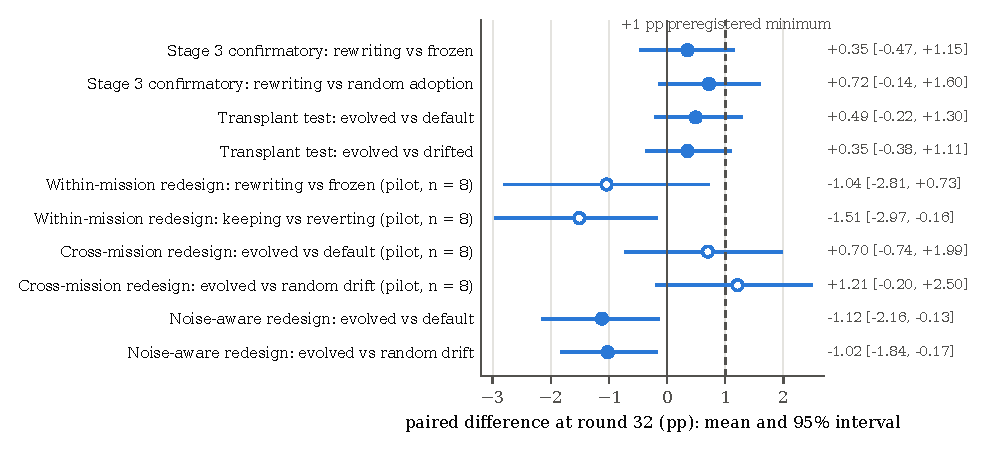
\includegraphics[width=\linewidth]{figures/fig2_causal_contrasts.pdf}
\caption{Every causal contrast across the five preregistered studies: round-32 paired difference, mean and bootstrap 95\% interval, from \cite{felix2026c3}, Figure 15. Filled markers: confirmatory ($n=24$); hollow: Gate 1 pilots ($n=8$). None meets its preregistered criterion.}
\label{fig:followups}
\end{figure}

After the confirmatory run, four further studies asked whether rewriting Imp can make the system a better improver at all, each with its own registered protocol, freeze, gates and unused seeds (Figure~\ref{fig:followups}).
\begin{itemize}
\item \textbf{Transplant test.} Each evolved Imp was frozen into a fresh mission and compared with the default Imp: $+0.49$ pp, $[-0.22, +1.30]$, $p = 0.17$. Fail.
\item \textbf{Within-mission validation.} A variant ran in a forked copy of the system and was judged on fresh tasks. The pilot gave $-1.04$ pp with power 0.00; 40\% of validations were exact ties, and keeping variants was worse than reverting them ($-1.51$ pp). NO-GO.
\item \textbf{Cross-mission validation.} A variant was judged over four whole missions on fresh seeds before adoption. The pilot gave $+0.70$ pp, the first design to beat both the default and random drift in direction, but with power 0.15. NO-GO.
\item \textbf{Noise-aware cross-mission validation.} A variant had to pass a four-seed screen and then win on eight never-reused seeds by a margin. Every adopted edit won its confirmation, yet on 24 fresh seeds the evolved mechanisms did worse than the default: $-1.12$ pp, $[-2.16, -0.13]$, $p = 0.97$. Fail.
\end{itemize}
An exploratory headroom scan explains the pattern: alternative fixed Imp settings held for whole missions were worth at most about $+1.6$ to $+2.1$ pp on four development seeds, against a per-seed standard deviation of paired differences of 2.1 pp, while a single audited promotion moves a mission by several points. If productive recursion exists in this system, it is smaller than evidence at this scale can resolve.

\subsection{The improvement that does happen transfers to real bugs}\label{sec:transfer}

\begin{figure}[t]
\centering
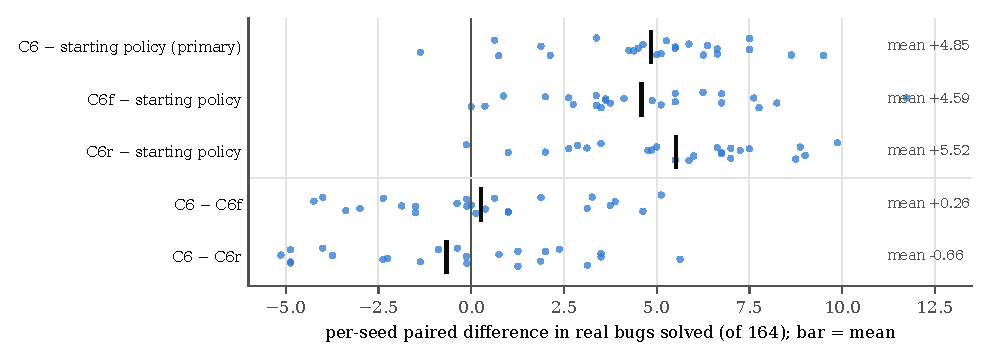
\includegraphics[width=\linewidth]{figures/fig3_transfer.pdf}
\caption{Transfer to 164 real bugs, per Stage 3 seed, from the printed per-seed table (\cite{felix2026c7}, Table 7). Every condition's end states beat the starting policy by about five bugs (top three rows); the conditions do not differ from each other (bottom two rows).}
\label{fig:transfer}
\end{figure}

All Stage 3 measurements were taken inside the synthetic domain the system trained on. A companion preregistered study \cite{felix2026c7} took the 72 confirmatory end states, verified each against the published audit manifest, and ran them unmodified through the same frozen repair search on 164 valid real bugs from QuixBugs \cite{lin2017quixbugs} (27) and HumanEvalFix \cite{muennighoff2024octopack} (137). The only new code was a sandboxed executor and a port of the search, which reproduced the original search exactly in 1,200 of 1,200 synthetic searches.

Under the identical budget, the C6 end states solved 25.81 bugs against 20.96 for the starting policy: $+4.85$ bugs, $[3.80, 5.84]$, 23 of 24 seeds improved, $p = 3.0\times10^{-7}$, a relative gain of 23\% against 47\% on the synthetic domain. The gain held at four times the training budget ($+2.17$, $p = 4.3\times10^{-4}$), vanished when the learned parameters were permuted (trained minus permuted $+5.97$, $p = 3.0\times10^{-7}$), and came entirely from HumanEvalFix ($+5.08$; QuixBugs $-0.23$). The three conditions transferred equally (C6 $-$ C6f $+0.26$, $p = 0.68$; C6 $-$ C6r $-0.67$, $p = 0.35$; Figure~\ref{fig:transfer}), and both findings replicated on 72 independent end states from the noise-aware study. The system is a one-step repairer that can reach at most 55 of the 164 bugs; these numbers should not be compared with general repair tools.

\section{Reanalysis and power}\label{sec:reanalysis}

\paragraph{Reproduction from printed tables.} We transcribed the per-seed tables of both papers into CSV files and recomputed the reported statistics with a standard-library script that implements the exact Wilcoxon procedure of \cite{felix2026c3}, Appendix C. Every reported mean, seed count and Imp-activity total is reproduced. The recomputed p-values agree closely despite rounding in the printed inputs: A-4 $7.63\times10^{-6}$ (reported $7.6\times10^{-6}$), B-2 0.081 (0.079), C7 primary $2.98\times10^{-7}$ ($3.0\times10^{-7}$), C7 budget-48 $4.1\times10^{-4}$ ($4.3\times10^{-4}$). B-1 gives 0.257 against the reported 0.23, a difference consistent with the 0.1 pp rounding of the printed rates.

\paragraph{Power.} Resampling the 24 B-1 differences (SD 2.06 pp) as a noise model and shifting them to an assumed true effect shows two things. First, the 24-seed design had about 50\% power even if the true benefit of recursion had been the full $+1.0$ pp; the Tier~B null therefore excludes large benefits but not modest ones, as the C3 paper states. Second, the rule ``$p < \alpha$ \emph{and} observed mean $\ge$ the minimum effect'' caps power near 57\% when the true effect equals that minimum, whatever the sample size, because the observed mean falls below it about half the time. Requiring significance plus an observed mean of at least half the target effect removes the cap: with 48 seeds it gives power 0.87 at a true $+1.0$ pp and 0.99 at $+1.5$ pp. We adopt this rule for the follow-up protocol.

\section{Discussion}\label{sec:discussion}

\paragraph{What the result establishes.} Under a protocol fixed before any code was written, the system proposes, validates and applies modifications without a human; rewrites its own improvement mechanism, adopting only variants that win a paired, budget-neutral trial; in most missions rewrites the very procedure that does the rewriting; and keeps improving on fresh test tasks through the second half of long missions. It meets Liu et al.'s Level-4 definition as operationalised here. It does not show that the recursion helps: the identical system without recursion does as well, on synthetic tasks and on real bugs.

\paragraph{Why the recursion was not productive.} Three observations point the same way. The rewritable parameters are worth little: about two points at best when held for a whole mission. The trial signal is weak: each trial compares four candidates per side over a few rounds, and a single promotion outweighs the few-round effect of any Imp setting. And the base loop is strong: every condition gains about 10.6 pp in the first half whatever Imp does. The follow-up studies sharpen the diagnosis: making validation stricter did not help, so the limit is the value of the rewritable parameters more than the way rewrites are validated.

\paragraph{A reporting standard for RSI claims.} A system can satisfy every clause of a role-based definition while its recursion is inert, so a classification by itself says little about capability. We suggest that claims of recursive self-improvement report, at matched budget:
\begin{enumerate}
\item a \textbf{frozen-mechanism control}: the same system with its improvement mechanism held fixed;
\item a \textbf{random-adoption control}: mechanism changes adopted without evidence on the same schedule;
\item a \textbf{power analysis} for the counterfactual contrast, stated before the result;
\item an \textbf{outside baseline}: a simple search method given the same evaluation budget;
\item \textbf{external transfer}: performance outside the training domain; and
\item \textbf{preregistration} of these comparisons, ideally on a public registry.
\end{enumerate}
This is the distinction Chen et al.\ draw between self-refinement against a fixed evaluator and recursion that closes the loop \cite{chen2026rsi}. In this system the policy-level validator is external and robust; the mechanism-level validator is internal, and that is where the signal is weakest.

\section{Limitations}

\begin{itemize}
\item \textbf{Operationalisation.} The criteria are our reading of a definition written to classify architectures; ``long-term'' could demand far longer horizons than 32 rounds, and ``rewrite its own improvement mechanism'' could be read as requiring code-level rewriting. Imp has a fixed schema of 11 parameters; the system changes their values but not the schema.
\item \textbf{An unreviewed standard.} Liu et al.\ and Chen et al.\ were unreviewed preprints when this study was registered.
\item \textbf{Power.} Tier~B was powered to fail, as the gate record predicted; its intervals exclude large benefits of recursion but not small ones.
\item \textbf{No outside baseline yet.} All conditions share the improvement loop; whether the loop beats a simple search at the same budget is untested (test T1 below).
\item \textbf{Test-task overlap.} In the development families, 73\% of test tasks on average share program text with some training task while carrying different examples; the overlap is identical across conditions but inflates absolute solve rates. Held-out families have none.
\item \textbf{Attestation and access.} The protocol and freeze, gate and results records were registered in a private document store with server timestamps, not a public registry. There is one implementation and no independent replication; source code and mission records are available to reviewers only under a confidentiality agreement.
\item \textbf{Scope.} One small synthetic domain; the transfer study reaches at most 55 of 164 real bugs. Nothing here speaks to systems built on large models.
\end{itemize}

\section{Planned tests}\label{sec:next}

We have drafted, but not yet run or registered, three follow-up studies. The draft, the power analysis and an analysis script that applies the decision rules are in the repository listed under Data and code availability. \textbf{T1} compares the improvement loop with a frozen Imp against a random-search proposer and a (1+8) evolution strategy at identical budget, screening and audit (24 seeds). \textbf{T2} bounds what any fixed Imp could be worth: 64 random Imp configurations plus the default are screened on 8 development seeds, and the best is confirmed against the default on 24 fresh seeds; if the upper 95\% limit is below $+1.0$ pp, rewriting Imp cannot clear the bar in this domain. \textbf{T3} repeats the Stage~3 comparison over 128 rounds with the training distribution changing at rounds 32, 64 and 96, the setting in which an adaptive mechanism has most room to help, with 48 seeds giving power 0.87 at a true $+1.0$ pp.

\section*{Data and code availability}

The repository \url{https://github.com/recurse-root/FRMDevelopment} (archived at DOI \href{https://doi.org/10.5281/zenodo.23366848}{10.5281/zenodo.23366848}) holds the source papers with checksums, the per-seed tables as CSV, the reanalysis script, the figure script for this article, the power analysis and the follow-up preregistration draft. The source papers are at DOIs \href{https://doi.org/10.5281/zenodo.23366534}{10.5281/zenodo.23366534} (C3) and \href{https://doi.org/10.5281/zenodo.23366502}{10.5281/zenodo.23366502} (C7). Frozen sources and mission records are held in audit packages, with SHA-256 hashes listed in the source papers, and are available to reviewers on request under a confidentiality agreement.

\section*{Use of AI assistance}

The research direction and the decisions to test against the published definition, to proceed, to publish and to disclose are the author's. Study design, implementation of the system and harness, execution and monitoring, statistical analysis, figures and drafting of the source papers and of this article were carried out with substantial assistance from an AI system (Claude, Anthropic) working under the author's direction. The AI is not part of the system under test: every self-modification reported here was proposed, validated and applied by the system itself.

\begin{thebibliography}{99}\small
\bibitem{good1966} I.~J. Good. Speculations concerning the first ultraintelligent machine. \emph{Advances in Computers}, 6:31--88, 1966.
\bibitem{schmidhuber2003} J.~Schmidhuber. G\"odel machines: Self-referential universal problem solvers making provably optimal self-improvements. Technical Report IDSIA-19-03, arXiv:cs/0309048, 2003.
\bibitem{zelikman2024stop} E.~Zelikman, E.~Lorch, L.~Mackey, and A.~T. Kalai. Self-Taught Optimizer (STOP): Recursively self-improving code generation. In \emph{COLM}, 2024. arXiv:2310.02304.
\bibitem{yin2025godel} X.~Yin, X.~Wang, L.~Pan, L.~Lin, X.~Wan, and W.~Y. Wang. G\"odel Agent: A self-referential agent framework for recursive self-improvement. In \emph{ACL}, 2025. arXiv:2410.04444.
\bibitem{hu2025adas} S.~Hu, C.~Lu, and J.~Clune. Automated design of agentic systems. In \emph{ICLR}, 2025. arXiv:2408.08435.
\bibitem{zhang2026dgm} J.~Zhang, S.~Hu, C.~Lu, R.~Lange, and J.~Clune. Darwin G\"odel Machine: Open-ended evolution of self-improving agents. In \emph{ICLR}, 2026. arXiv:2505.22954.
\bibitem{robeyns2025sica} M.~Robeyns, M.~Szummer, and L.~Aitchison. A self-improving coding agent. arXiv:2504.15228, 2025.
\bibitem{wang2026hgm} W.~Wang, P.~Pi\k{e}kos, L.~Nanbo, F.~Laakom, Y.~Chen, M.~Ostaszewski, M.~Zhuge, and J.~Schmidhuber. Huxley-G\"odel Machine: Human-level coding agent development by an approximation of the optimal self-improving machine. In \emph{ICLR}, 2026. arXiv:2510.21614.
\bibitem{liu2026path} S.~Liu, Z.~Lin, Y.~Zhang, Y.~Ren, Y.~Wu, Y.~Li, Z.~Wang, Z.~Fu, and J.~Ye. The path to recursive self-improving agents: Foundation, framework, and future directions. Preprints.org, preprint 202608.0051, version 1, 2026. Not peer reviewed.
\bibitem{chen2026rsi} M.~Chen, L.~Wang, and B.~Qu. Recursive self-improvement in AI: From bounded self-refinement to autonomous research loops. arXiv:2607.07663, 2026.
\bibitem{yampolskiy2015} R.~V. Yampolskiy. From seed AI to technological singularity via recursively self-improving software. arXiv:1502.06512, 2015.
\bibitem{andrychowicz2016} M.~Andrychowicz, M.~Denil, S.~G\'omez Colmenarejo, M.~W. Hoffman, D.~Pfau, T.~Schaul, B.~Shillingford, and N.~de Freitas. Learning to learn by gradient descent by gradient descent. In \emph{NeurIPS}, 2016. arXiv:1606.04474.
\bibitem{real2020automl} E.~Real, C.~Liang, D.~R. So, and Q.~V. Le. AutoML-Zero: Evolving machine learning algorithms from scratch. In \emph{ICML}, 2020. arXiv:2003.03384.
\bibitem{nosek2018} B.~A. Nosek, C.~R. Ebersole, A.~C. DeHaven, and D.~T. Mellor. The preregistration revolution. \emph{PNAS}, 115(11):2600--2606, 2018.
\bibitem{henderson2018} P.~Henderson, R.~Islam, P.~Bachman, J.~Pineau, D.~Precup, and D.~Meger. Deep reinforcement learning that matters. In \emph{AAAI}, 2018. arXiv:1709.06560.
\bibitem{pineau2021} J.~Pineau, P.~Vincent-Lamarre, K.~Sinha, V.~Larivi\`ere, A.~Beygelzimer, F.~d'Alch\'e-Buc, E.~Fox, and H.~Larochelle. Improving reproducibility in machine learning research. \emph{JMLR}, 22(164):1--20, 2021.
\bibitem{wilcoxon1945} F.~Wilcoxon. Individual comparisons by ranking methods. \emph{Biometrics Bulletin}, 1(6):80--83, 1945.
\bibitem{efron1979} B.~Efron. Bootstrap methods: Another look at the jackknife. \emph{The Annals of Statistics}, 7(1):1--26, 1979.
\bibitem{candea2003} G.~Candea and A.~Fox. Crash-only software. In \emph{HotOS IX}, USENIX, 2003.
\bibitem{demillo1978} R.~A. DeMillo, R.~J. Lipton, and F.~G. Sayward. Hints on test data selection: Help for the practicing programmer. \emph{Computer}, 11(4):34--41, 1978.
\bibitem{jia2011} Y.~Jia and M.~Harman. An analysis and survey of the development of mutation testing. \emph{IEEE TSE}, 37(5):649--678, 2011.
\bibitem{lin2017quixbugs} D.~Lin, J.~Koppel, A.~Chen, and A.~Solar-Lezama. QuixBugs: A multi-lingual program repair benchmark set based on the Quixey challenge. In \emph{SPLASH Companion}, pages 55--56, 2017.
\bibitem{muennighoff2024octopack} N.~Muennighoff, Q.~Liu, A.~Zebaze, Q.~Zheng, B.~Hui, T.~Y. Zhuo, S.~Singh, X.~Tang, L.~von Werra, and S.~Longpre. OctoPack: Instruction tuning code large language models. In \emph{ICLR}, 2024. arXiv:2308.07124.
\bibitem{felix2026c3} J.~P. Felix. Level-4 bounded recursive self-improvement under a published definition: A preregistered test of a self-referential improvement mechanism. Version 1.3. Zenodo, 2026. doi:10.5281/zenodo.23366534.
\bibitem{felix2026c7} J.~P. Felix. Do self-improved repair policies transfer to real bugs? A preregistered external-benchmark test of a Level-4 bounded self-improving system. Version 1.1. Zenodo, 2026. doi:10.5281/zenodo.23366502.
\end{thebibliography}

\end{document}
